\chapter{Assignment 2: Basic Probabilities and Visualizations}

\section{Task a}
For the given samples (Variable X and Y) a scatter plot deems to be the most suitable candidate to plot the given points. This can be said because scatter plot helps to show the relationship between two variables, as one can see where the different points lie in the graph. This tells us how co-related the samples are.

\begin{figure}[h!]
\centering
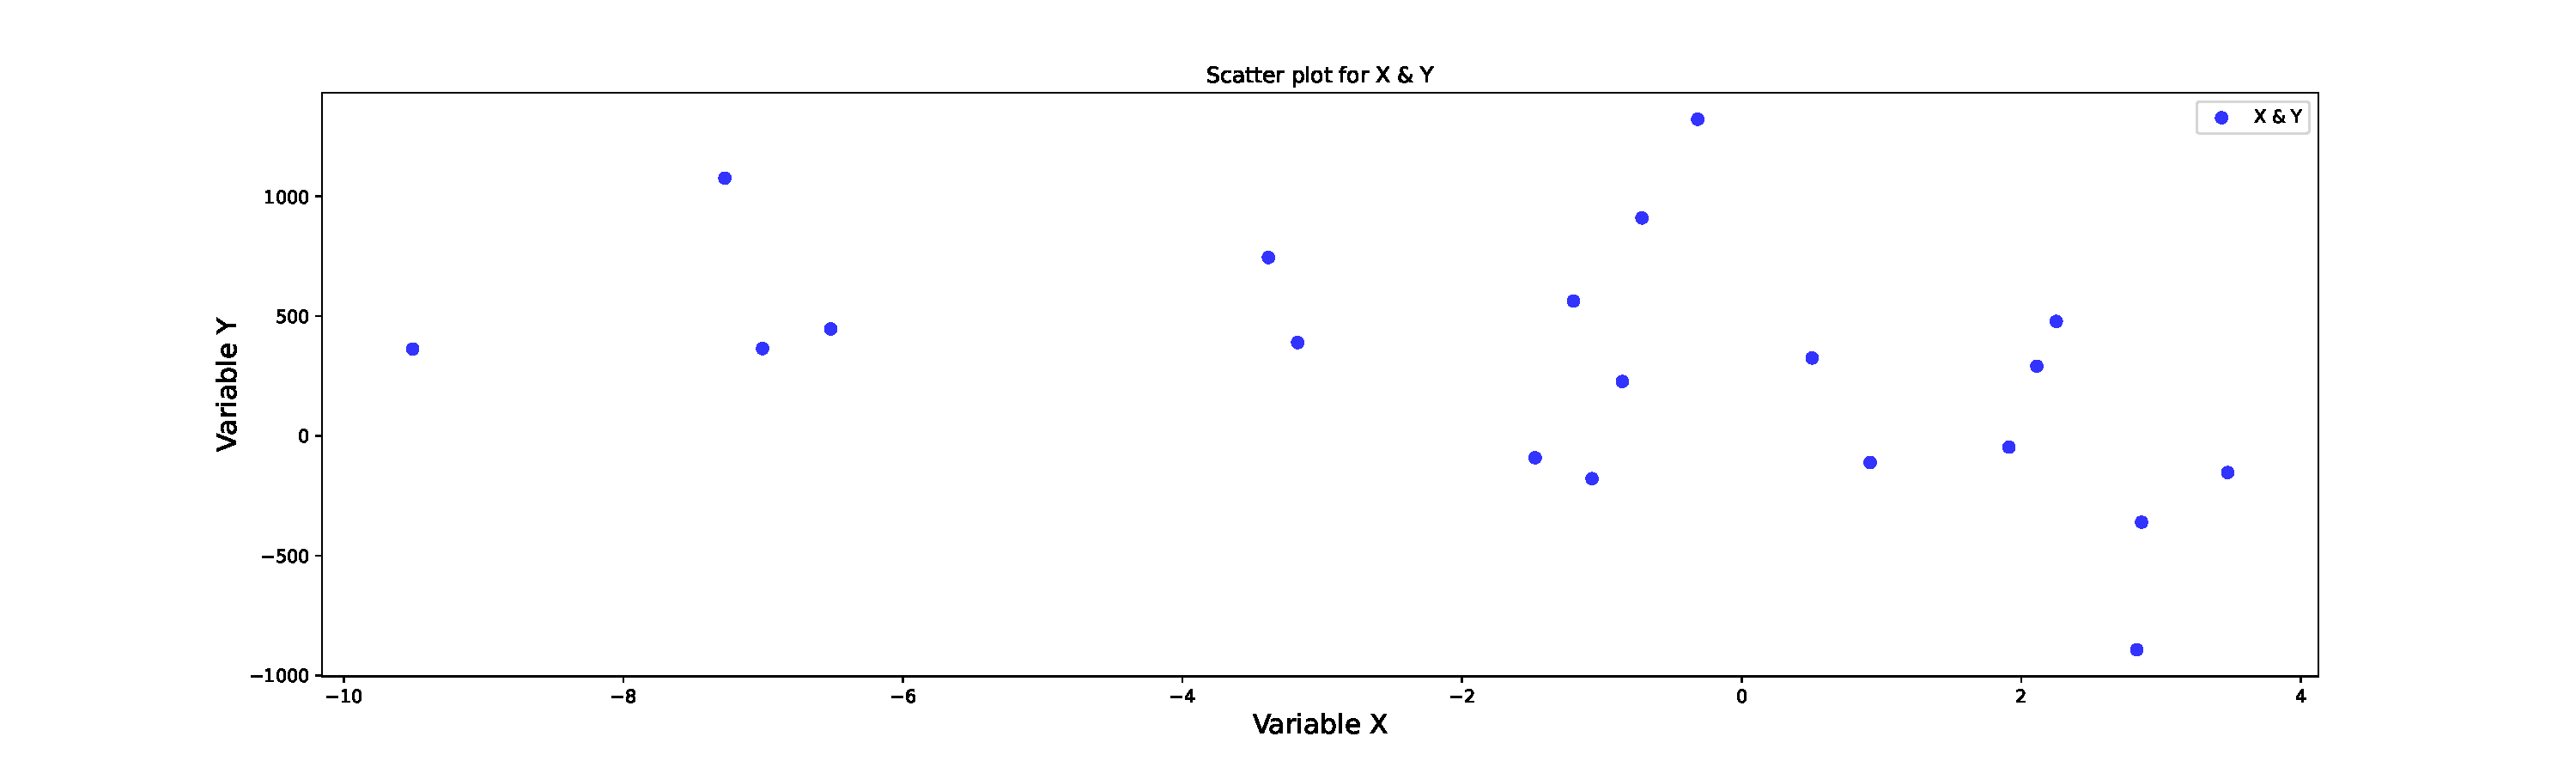
\includegraphics[width=\textwidth]{pics/task_2_a.pdf}
\caption{Scatter Plot for X and Y}\label{fig:task_2_a}
\end{figure}
\FloatBarrier
\newline 
A simple look in the scatter plot (fig:\ref{fig:task_2_a}) shows us the data have a very large covariance as the points in the graph are very sparsely distributed in the plot.

\begin{lstlisting}[caption={Plotting the Scatter Plot with Variance Calculations)},label={lst:code_task_2_a}]
import numpy as np
import matplotlib.pyplot as plt

# Definitions
sample_data = [(-1.202, 563.024), (2.112, 291.072), (2.827, -893.619), (-0.314, 1321.814),
               (-1.477, -91.573), (-6.516, 446.336), (0.920, -111.487), (3.477, -153.165),
               (-7.273, 1076.221), (2.251, 477.931), (-0.713, 909.696), (-0.853, 226.865),
               (-3.176, 389.413), (1.913, -47.169), (-1.070, -178.695), (-3.385, 744.486),
               (-9.506, 362.670), (-7.004, 364.578), (0.504, 324.975), (2.861, -360.571)]

# Plot the probability distribution
fig, ax = plt.subplots(1, 1, figsize=(20, 6))
# Separate value of X and Y from sample data
x, y = zip(*sample_data)

plt.scatter(x, y, color='b', label='X & Y', alpha=0.8)
plt.title('Scatter plot for X & Y')
plt.xlabel('Variable X', fontsize=15)
plt.ylabel('Variable Y', fontsize=15)

# Mean and covariance
mean_x = sum(x) / len(x)
mean_y = sum(y) / len(y)
x_minus_mean_x = np.asarray(x) - mean_x
y_minus_mean_y = np.asarray(y) - mean_y
# Covariance of X & Y
cov_x_y = sum(x_minus_mean_x * y_minus_mean_y) / len(x)
# Variance of X
var_x = sum(np.power(x_minus_mean_x, 2)) / len(x)
# Variance of Y
var_y = sum(np.power(y_minus_mean_y, 2)) / len(y)

plt.legend()
plt.savefig('images/task_2_a.pdf')
\end{lstlisting}

\subsubsection{Mean \& Covariance}   

The mean of Variables can be calculated using E[X]=  $\frac{1}{N} \sum_{i=1}^{N}x_i$  (\cite{Iubh:2021}) where N=20 is the total number of samples and the numerator is the sum of the random variable X or Y. Using this formula, the expectation ($\mu$) of the variable X and Y are calculated. E[X] = $\mu_x$= -1.28 and E[Y] = $\mu_y$= 283.14.\newline 
The Covariance of two variables can be calculated using cov(X,Y) =  $\frac{1}{N} \sum_{i=1}^{N}(x_i - \mu_x)^2 (y_i - \mu_y)$ (\cite{Iubh:2021}). Using the given formula, the cov(X,Y)= -863.73

Similarly, the Variance can be calculated using var[X]=$\frac{1}{N} \sum_{i=1}^{N}(x_i - \mu_x)^2$. The calculated variances are as follows Var[X]=13.60 and Var[Y]= 2.6e+5.

\subsection{Task b}
